\documentclass[11pt]{standalone}
\usepackage{tikz}
\begin{document}
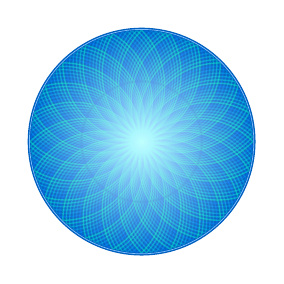
\begin{tikzpicture}[line width=.5pt]
  \shade [draw=blue!50!cyan!75!black, line width=.5pt, double distance=.25pt, 
  double=blue!50!cyan!50!white, inner color=blue!50!cyan!25!white,
  outer color=blue!50!cyan!75!black, opacity=1, draw opacity=1] (0,0) circle (1.425);
  \begin{scope}[blend mode=screen, opacity=.5]
    \clip (0,0) circle (1.415);
    \foreach \k [count=\c, evaluate=\c as \f using {\c*100/7}] in {0,2.5,5,...,12.5}
    {\begin{scope}[rotate=\k]
        \foreach \j in {0,15,30}
        {
          \scoped[rotate=\j]{
            \draw [blue!\f!green] \foreach \i in {0,45,...,315} { (\i:1) circle (1) };
          }
        }
      \end{scope}
    }
  \end{scope}
\end{tikzpicture}
\end{document}
